\documentclass{beamer}
\usepackage[utf8]{inputenc}
\usepackage{graphicx}
\author[Sowmya Vajjala]{Instructor: Sowmya Vajjala}


\title[LING 120]{LING 120: \\ Language and Computers}
\subtitle{Semester: Fall 2017}

\date{8 September 2017}

\institute{Iowa State University, USA}

%%%%%%%%%%%%%%%%%%%%%%%%%%%

\begin{document}

\begin{frame}\titlepage
\end{frame}

\begin{frame}
\frametitle{Class Outline}
\begin{enumerate}
\item Last class' question
\item Context sensitive spelling correction
\item Assignment 2 description
\end{enumerate}
\end{frame}

\begin{frame}
\frametitle{Question from last class}
Visit \url{www.eogn.com/soundex/} and list a few examples of where Soundex will fail. Use some non-word errors and their correct versions and check which pairs have the same soundex and which pairs don't. Try to come up with 2 examples for each case and analyse why are the soundex codes same or different.
\\ Example: Assignment can have two mis-spellings (among others). Asignment, Assingment - First one will have the same soundex as the original word. Second one won't have. Why? (sounds are different)
\end{frame}

\begin{frame}
\frametitle{Your Answers}
\begin{enumerate}
\item Cases where Soundex will work and show a correct alternative:
\begin{itemize}
\item  Calculate, calculade (C-424); Discussion-Discusion (D-225)
\pause \item But, there are also these false positives that can come up: Discussion-Decagon (D225!)
\\ (for more such false positive examples, check out: \url{https://goo.gl/2sz3yW}) 
\end{itemize} \pause
\item Cases where Soundex will not work: 
\begin{itemize}
\item Discussion-Discssion (D-225, D-250)
\item laf, laugh - L100 and L200
\item night, nite - N-230, N-300
\end{itemize}
\item Another major problem: For long words, you may never get right suggestions (Why?) \pause
Revolution, Revolutionize, Revolutionary, Revolutionist, Revolutionization- all get the same Soundex! 
\end{enumerate}
\end{frame}

\begin{frame}
\frametitle{}
\begin{center}
\Large Today's topic: Context Sensitive Spelling Correction
\end{center}
\end{frame}

\begin{frame}
\frametitle{What is the problem to solve?}
\begin{itemize}
\item ... detecting and correcting real word spelling errors.
\item i.e., words are not spelt wrong - they are spelt wrong in that context.
\item Grammar checking is considered a context sensitive spelling correction process.
\item Since everything is dependent on context, can we say every word is a potential error? (What? How?)
\end{itemize}
\end{frame}

\begin{frame}
\frametitle{Some examples}
\begin{itemize}
\item Let us take this sentence: "There house is nice". There are two possible "correct" options.
\begin{itemize}
\item The house is nice.
\item Their house is nice. (more likely)
\item The house there is nice. 
\end{itemize}
\item Or another: "The teams was successful". There are again two possible "correct" options.
\begin{itemize}
\item The team was successful.
\item The teams were successful. (can we say for certain what is more likely?)
\end{itemize}
\item How does a computer go about detecting such errors?
\end{itemize}
\end{frame}

\begin{frame}
\frametitle{What are the causes of contexual word errors?}
\begin{itemize}
\item "False Friends": \textit{bekommen} in German means \textit{get}. So, a German native speaker, when writing English may confuse between become and get. \pause
\item Words sound the same: their vs there. \pause
\item Influence of the sentence structure in the writer's native language (many Indian English speakers make errors with articles because several languages do not have them).  \pause
\item Not knowing the rules of the language (e.g., subject-verb agreement. \textit{He has} but not \textit{He have} \pause
\item Gender errors due to native language background (e.g, one language has the Gender for Sun as male. The other one has female.)
\end{itemize}
...
\end{frame}

\begin{frame}
\frametitle{Correcting such errors}
\begin{itemize}
\item Grammar based word correction
\item Error pattern based word correction
\item Probability based word correction
\item Meaning based word correction
\end{itemize}
\end{frame}

\begin{frame}
\frametitle{Grammar based word correction}
\begin{itemize}
\item Idea: encode the rules of language into a computer program. As the program tries to build a syntactic structure of the language, if there is no matching grammar rule, then it breaks, which is an indication that the sentence has an error.
\item \pause This is what I mean when I said "syntactic structure".
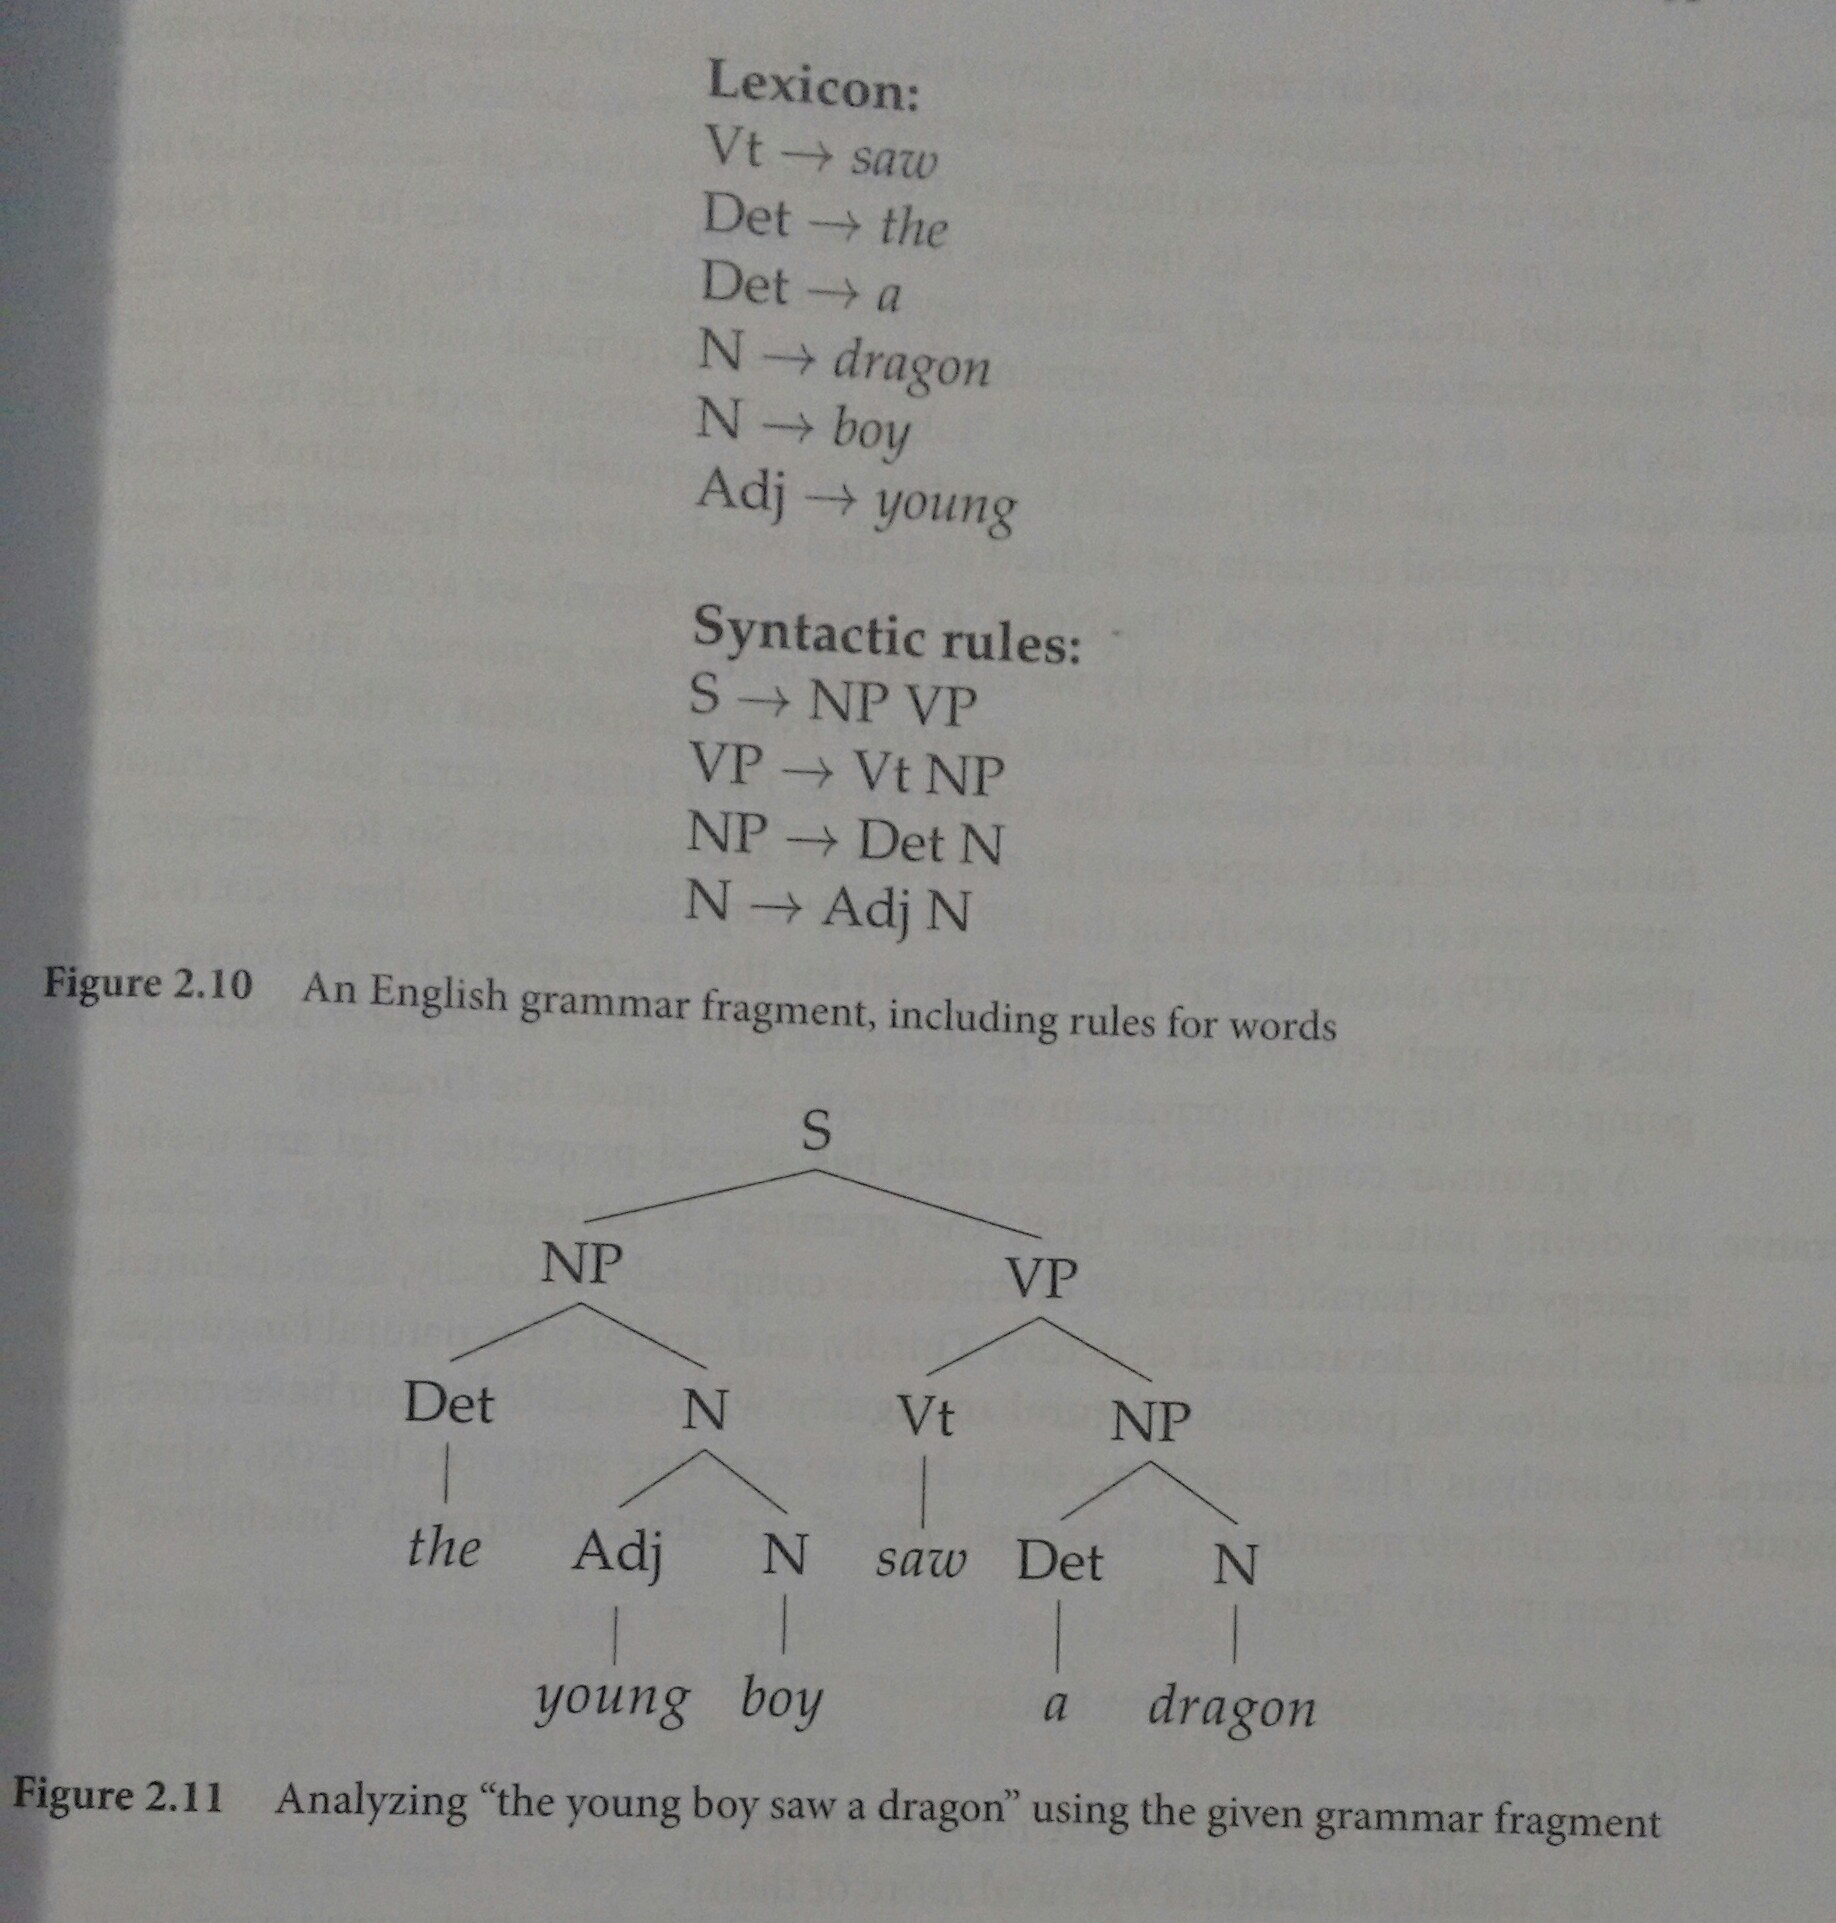
\includegraphics[width=0.5\textwidth]{parse.jpg}
\end{itemize}
\end{frame}

\begin{frame}
\frametitle{Pros and Cons}
\begin{itemize}
\item Pros: Very effective - specific error identification and feedback is possible.
\item Cons: Such a grammar has to be painstakingly prepared first, and suiting to the needs of a computational approach (which is time consuming and expensive)
\item Language is continuously changing - so new expressions, new syntactic structures keep coming. This approach will not work if we don't keep updating.
\end{itemize}
\end{frame}

\begin{frame}
\frametitle{Error pattern based word correction}
\begin{itemize}
\item Idea: Prepare a large set of rules of error patterns in language. Whenever there is a match to a rule, flag an error and suggest a solution (e.g. rule: if a plural word is followed by \textit{is}, flag an error, and suggest using \textit{are} instead). \pause
\item Pros: As long as we know what kind of errors the users make, this is a straight forward and effective process
\item Cons: Rule making takes time and expertise and money. Again, may be it is difficult to exhaustively cover every single error pattern.
\item However, all spell checkers you use today have some kind of a rule-engine inside it, along with something based on an n-gram approach.
\end{itemize}
\end{frame}

\begin{frame}
\frametitle{Probability based word correction}
\begin{itemize}
\item Idea: use frequencies of word n-grams in a large collection of texts to estimate what are the likely and unlikely n-grams in the language. \pause
\item E.g, Let us take this sentence: "John came form the house".
\item Since we don't know what word is an error in this context, let us start with the assumption that each word is a potential error.
\item Candidate words: let us leave John (poor guy!). Came - come, lame, tame, tame, cane etc; form: from, dorm, norm etc.; house - hos
\end{itemize}
\end{frame}

\begin{frame}
\frametitle{getting from word level candidates to sentence level suggestions}
\begin{itemize}
\item Try to make sentences with all these possible candidates replacing one candidate word at a time.
\item From a large corpus of English texts, estimate the likelihood of seeing each sentences (probability)
\item The sentence with highest probability gets the top-rank in suggestion list.
\end{itemize}
\end{frame}

%Pros and cons
\begin{frame}
\frametitle{Pros and Cons}
\begin{itemize}
\item Pros: Works around the problem of writing a lot of language specific rules which requires time and effort. 
\item Cons: Lot of calculations with large corpus-computationally intensive! (thankfully, computer programs have efficient way of organizing and retrieving data)
\item Cons: No direct way to handle unknown words or phrases 
\end{itemize}
Note: Real life spelling and grammar checkers use a combination of error pattern based and probability based methods.
\end{frame}

\begin{frame}
\frametitle{Meaning based word correction}
\begin{itemize}
\item Idea: Find words that do not fit into the meaning of the rest of the sentence. Replace them with words that are "semantically appropriate"
\item e.g., "It is my sincere \textit{hole} that you will recover swiftly" - hole seems semantically inappropriate.
\item "hope" suits better here. 
\item Problem: How do you choose the related word given a context? - this is studied in natural language processing under something called "distributional representation of language".
\end{itemize}
\end{frame}

\begin{frame}
\frametitle{Assignment 2 Description}
\begin{itemize}
\item Two questions - one each on isolated and contextual spelling correction
\item Requires you to analyze what the word processor tools show you and interpret the causes of the errors and suggestions.
\item Carries 10 marks.
\item Guidelines are on Canvas. 
\item Deadline: 23 September 2017
\end{itemize}
\end{frame}

\begin{frame}
\frametitle{Next Week}
\begin{itemize}
\item Topic 3: Language Tutoring Systems
\item Readings: Chapter 3 from the Textbook
\item Reminder: Submit Assignment 1!
\end{itemize}
\end{frame}

\begin{frame}
\frametitle{Attendance Question for today}
Write answers to any two of these scenarios on a sheet of paper and return it to me with your name on it. 
\begin{itemize}
\item 2 examples of grammar errors caused due to a change in word order
\item 2 examples of grammar errors caused due to usage of wrong tense
\item 2 examples of grammar errors caused because of gender-differences between the author's native language and English
\item 2 examples of using similar sounding words instead of each other (e.g., their-there, hole-whole -now, don't use these examples!)
\end{itemize}
\end{frame}

\end{document}
